\chapter{Analysis framework}

In order to study the Particle Flow jet performance and the data-MC comparison a large amount of ingredients is needed to be included and checked to be correctly working. This chapter covers the important tools included in the analysis framework. The impact of every given tool was studied and the status of the framework as well as possible problems in the current implementation are included.
The chapter starts with the event selection. The second section describes the trigger system and its corresponding tools and finally introduces the calibration tools for specific objects.

The final section describes the tools still to be implemented to achieve a better matching of data and Monte Carlo.




\section{Selection of good events}

The event selection is applied to mostly remove bad or corrupted data. The tools used are summarized below.

\subsection{The Good Run List}

Before any analysis or calibration takes place the Good Run List (GRL) has to be applied. The Good Run List is needed for data but not for Monte Carlo.

For data to be suitable for analysis one has to make sure that it fits certain requirements on the detectors working state. The Good Run List allows to exclude data-taking periods during which the detector showed a poor data quality. Reasons for this may be maintenance on sub detectors, magnets off or ramping or an unstable beam of the LHC.
The Good Run List includes all the good data taking periods.
For the data analysis in this thesis the recommended GRL for 2016 data was used.

Figure \ref{fig:datacuts} shows the number of events removed due to several cuts in the framework. The cuts due to the GRL are shown in the second bin. In this case no or at least very few events were removed due to the GRL. Depending on the data used the amount of events removed can be way higher.


\begin{figure}[h]
\centering
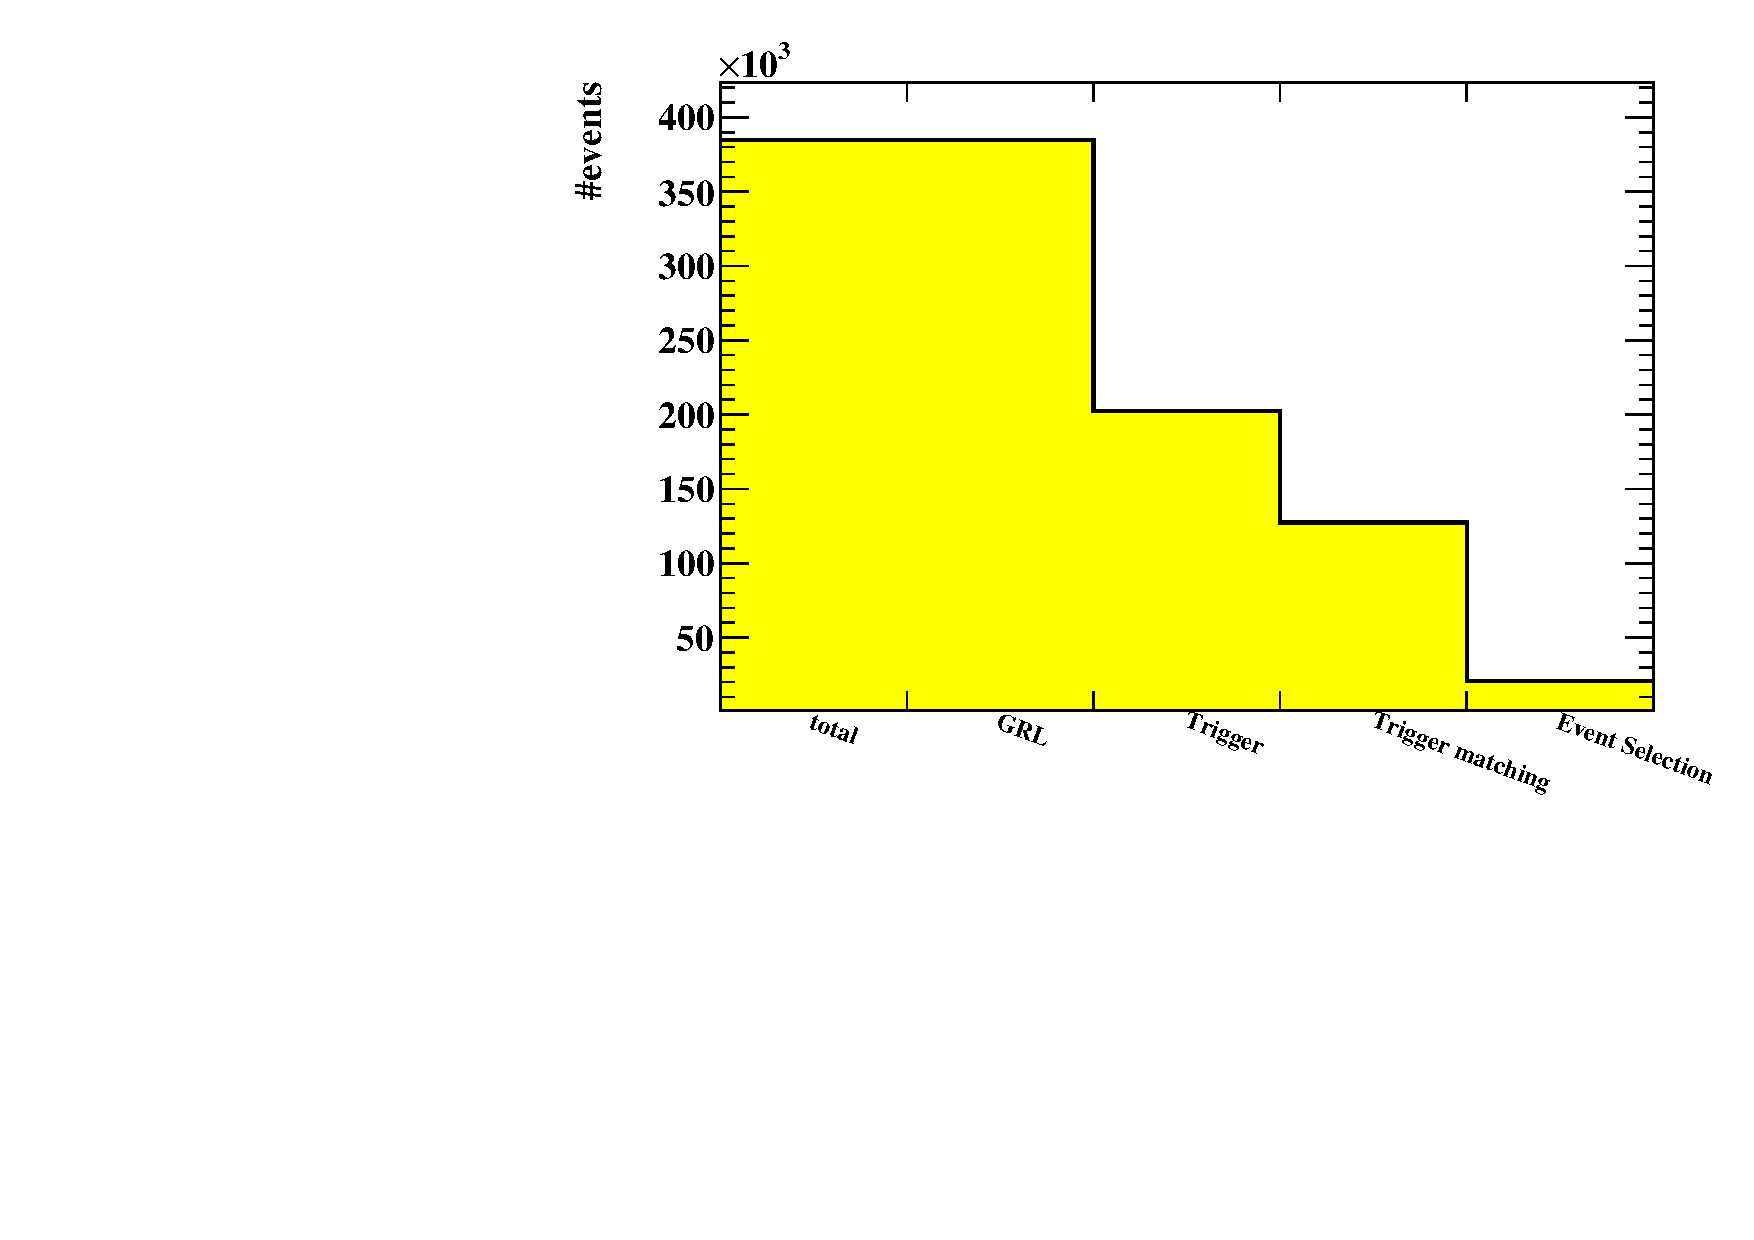
\includegraphics[scale=0.7]{datacuts}
\caption[Fraction of events removed due to the GRL, trigger, trigger matching and event selection]{Fraction of events removed due to the GRL, trigger, trigger matching and event selection. The amount of events removed due to the GRL is very minimal for the used dataset and not visible in this figure.}
\label{fig:datacuts}
\end{figure}



\subsection{Event cleaning}

Additionally to the cuts provided by the GRL some further events have to be excluded. Noise bursts and corrupted data in general have to be removed in the LAr, the SCT and the Tile. Furthermore due to production errors some events are duplicate and therefore have to be removed also. 


\section{Trigger Tools}

The trigger system makes sure that only the events that are interesting for physics analysis are kept.
A further important collection of tools has to make sure that the trigger is fired, correctly used and additionally that the particle that triggered is actually one of those used in further analysis.


\subsection{Trigger system}


A trigger basically is a first selection for an event meaning that an event is required to surpass certain demands to be used in analysis. These demands are embodied by so called trigger chains that can be used as input for a trigger tool in analysis which on that base can select or refuse events. For the analysis in this thesis the recommended single lepton triggers for 2016 data were used. The chains were HLT\_mu26\_ivarmedim, HLT\_mu50. As an example the first chain is briefly xplained here. HLT refers to the used trigger system level, mu26 means that muons with a minimum transverse momentum of \SI{26}{\GeV} are triggered on and  ????







\subsection{Trigger matching}

A trigger system preselects the events interesting for analysis. Depending on the events of interest there are different triggers setting the criteria on which events are preselected.

Usually the trigger is checked before the event is further cleaned and calibrated. Therefore it can happen that the particles having passed the trigger later get removed in the analysis. The trigger matching assures that the particles that have passed the triggers are still left in the final analysis and if not the event can still be removed.

\section{Monte Carlo Re-weighting and scale factors}

The Monte Carlo is produced before data is taken, why the simulation may vary from the data for several reasons. For example the pileup distribution used to generate the MC may not match the one in data. Pileup can occur in particle collision experiments if several events overlap. There is space and time pileup. In the case of in time pileup two events happen at the same time and in space pileup refers to secondary vertices. In both cases it is important to distinguish objects from the event of interest and those originating from pileup.

To compensate these differences a sum of weights is applied to Monte Carlo as well as to data.

The most general weights are the Monte Carlo event weight and the pileup re-weighting. Nevertheless there are numerous scale factors to be applied to all kind of objects. Jets, electrons, muons, tauons and photons all require scale factors to match the data. 

All these scale factors have to be multiplied and added as a weight to each event in both data and simulation to optimize the agreement between data and Monte Carlo as far as possible.

The current framework only includes the Monte Carlo weight and the pileup re-weighting. The other weights are going to be included in future updates of the framework development. Anyhow the changes expected from the missing scale factors are assumed to be rather small and do not exclude the results of this work from being significant.

\section{Object calibration and selection}

The last step in the framework is the selection and calibration of the objects per event. This section summarizes the tools needed not only for jets but also for muons and electrons, which are the objects present in our event topology.

\subsection{Jet cleaning}

The jet cleaning is applied to identify bad jets. Bad jets are jets not associated to real energy deposits in the calorimeters. They can occur due to a broad range of reasons: hardware problems, LHC beam condition or even cosmic-ray showers.

The Jet Cleaning is used on both data and Monte Carlo to make sure that Monte Carlo events that would be removed in data are also not included in the simulation.
Bad jets are excluded on the base of some of their properties: negative energy, charged fraction and energy deposited in specific calorimeter layers. The set of criteria is rather big and more information can be obtained in the twiki for example at \cite{jetcleaning}.

Jet cleaning variables are not yet available for Particle Flow jets and the cleaning has to be performed on topo-jets at the current state of the framework. If a bad topo-jet is found the whole event is removed from the analysis.
For this framework a "loose" \cite{jetcleaning} selection has been chosen since it is generally recommended.

\subsection{Jet Calibration and Smearing}

After making sure a jet is "good" and therefore has passed the cleaning it must still be be calibrated and in case of MC smeared to data. The calibration scales the energy of jets for a certain reconstruction algorithm. The Smearing smears the MC resolution to be matching the actual data resolution.

Figure \ref{jetsmearingandcalibration} shows the impact of these tools on the energy and the momentum of jets in a Monte Carlo sample.


\begin{figure}
\centering
\begin{subfigure}[b]{0.5\figwidth}
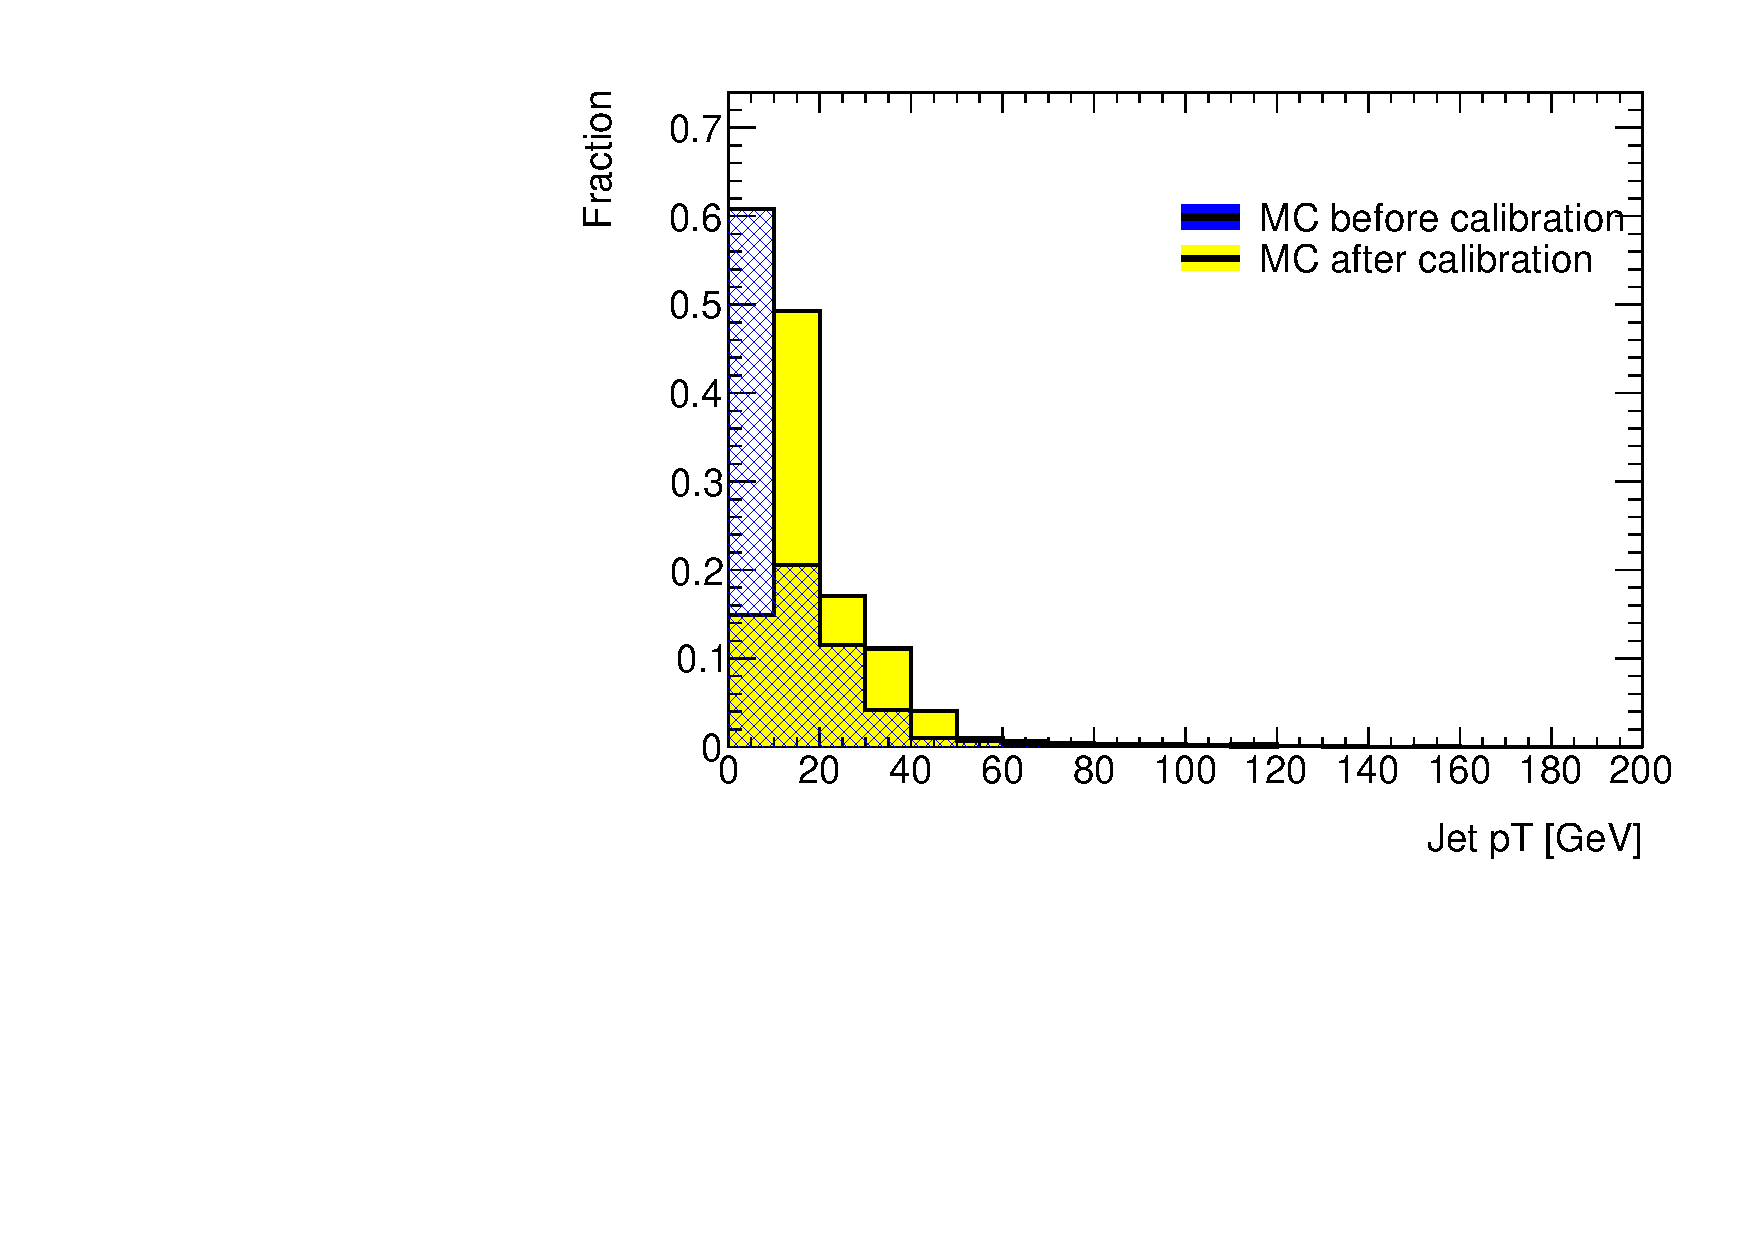
\includegraphics[width=0.53\figwidth]{testscalingpt}
\caption[Influence of the JES on the transverse momentum]{The influence of the calibration in momentum is shown}
\label{fig:testscalingpt}
\end{subfigure}
\quad
\begin{subfigure}[b]{0.5\figwidth}
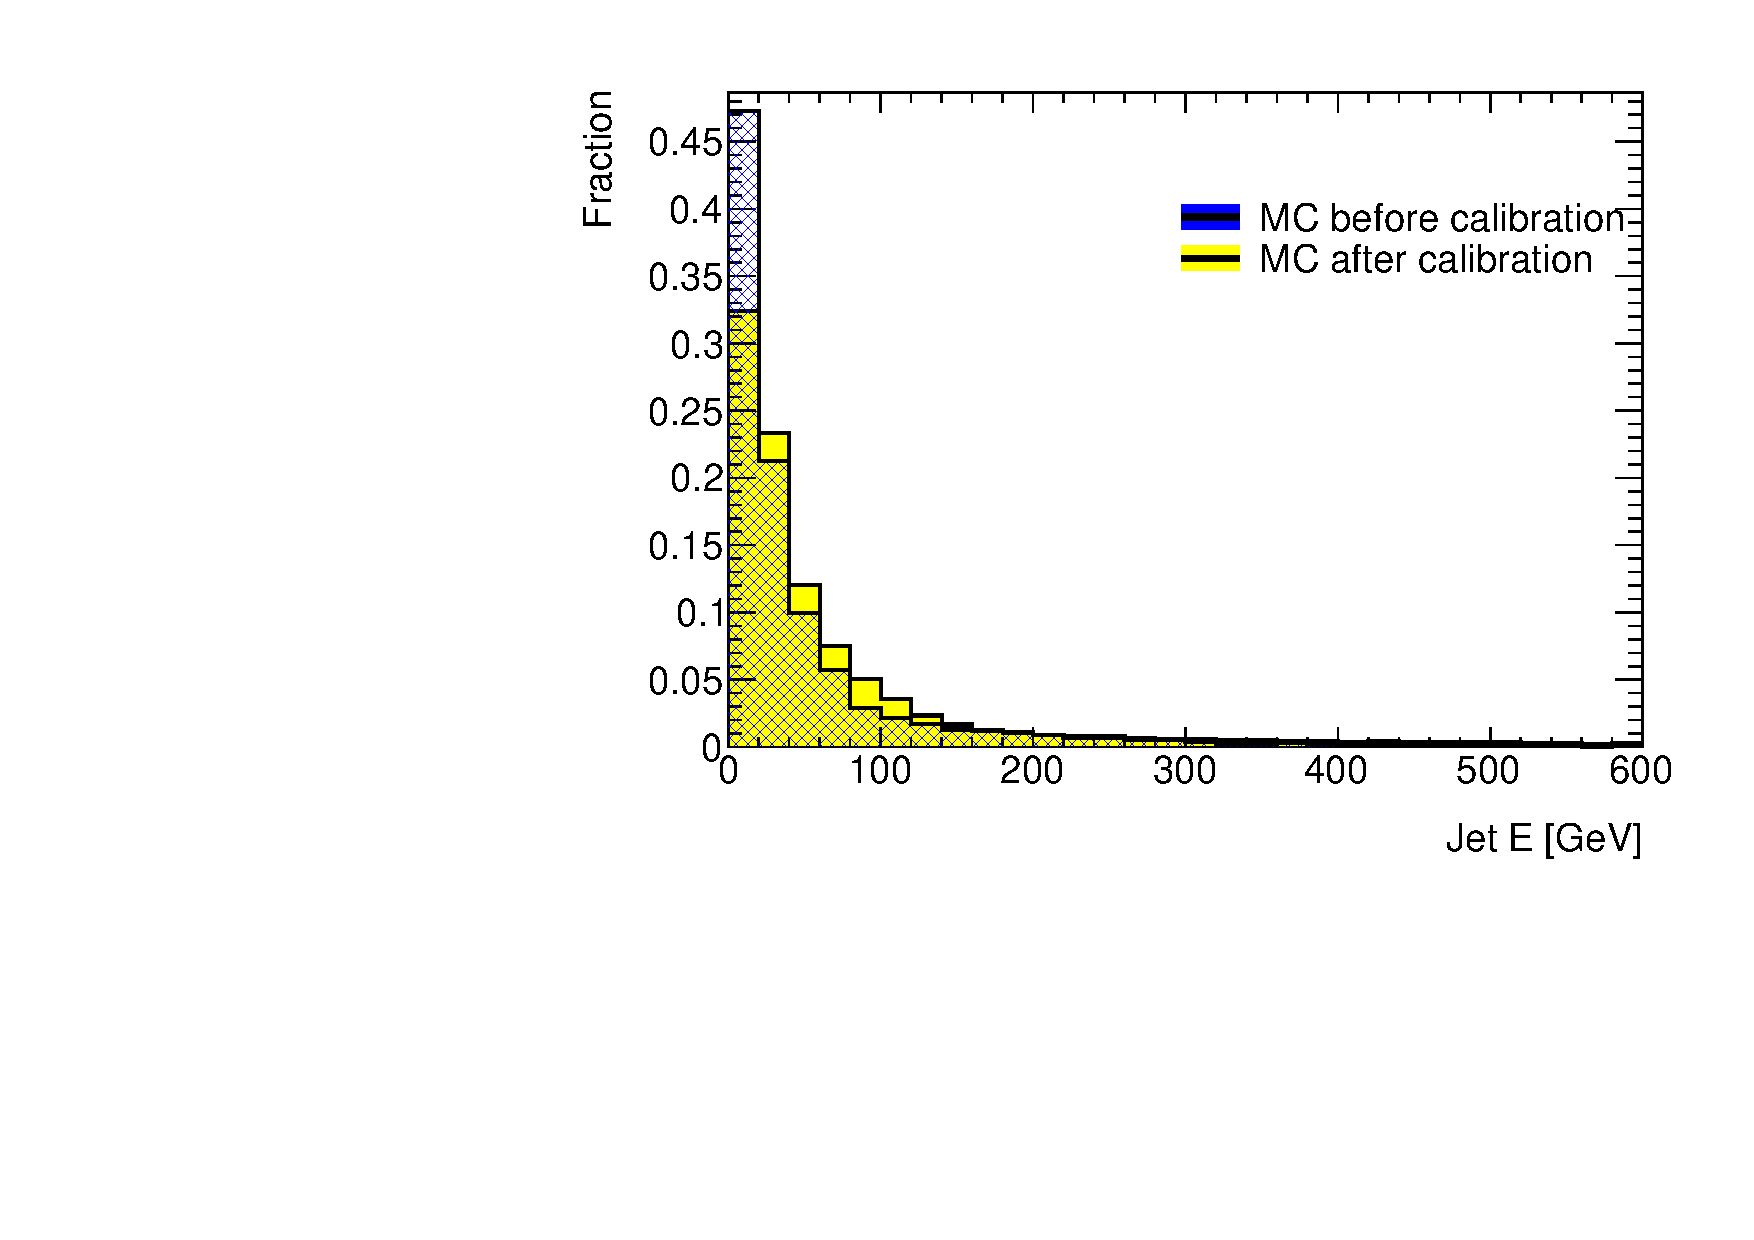
\includegraphics[width=0.53\figwidth]{testscalinge}
\caption[Influence of the JES on the energy]{The influence of the calibration in energy is shown}
\label{fig:testscalinge}
\end{subfigure}
%\end{figure}


%\begin{figure}
%\centering
\begin{subfigure}[b]{0.5\figwidth}
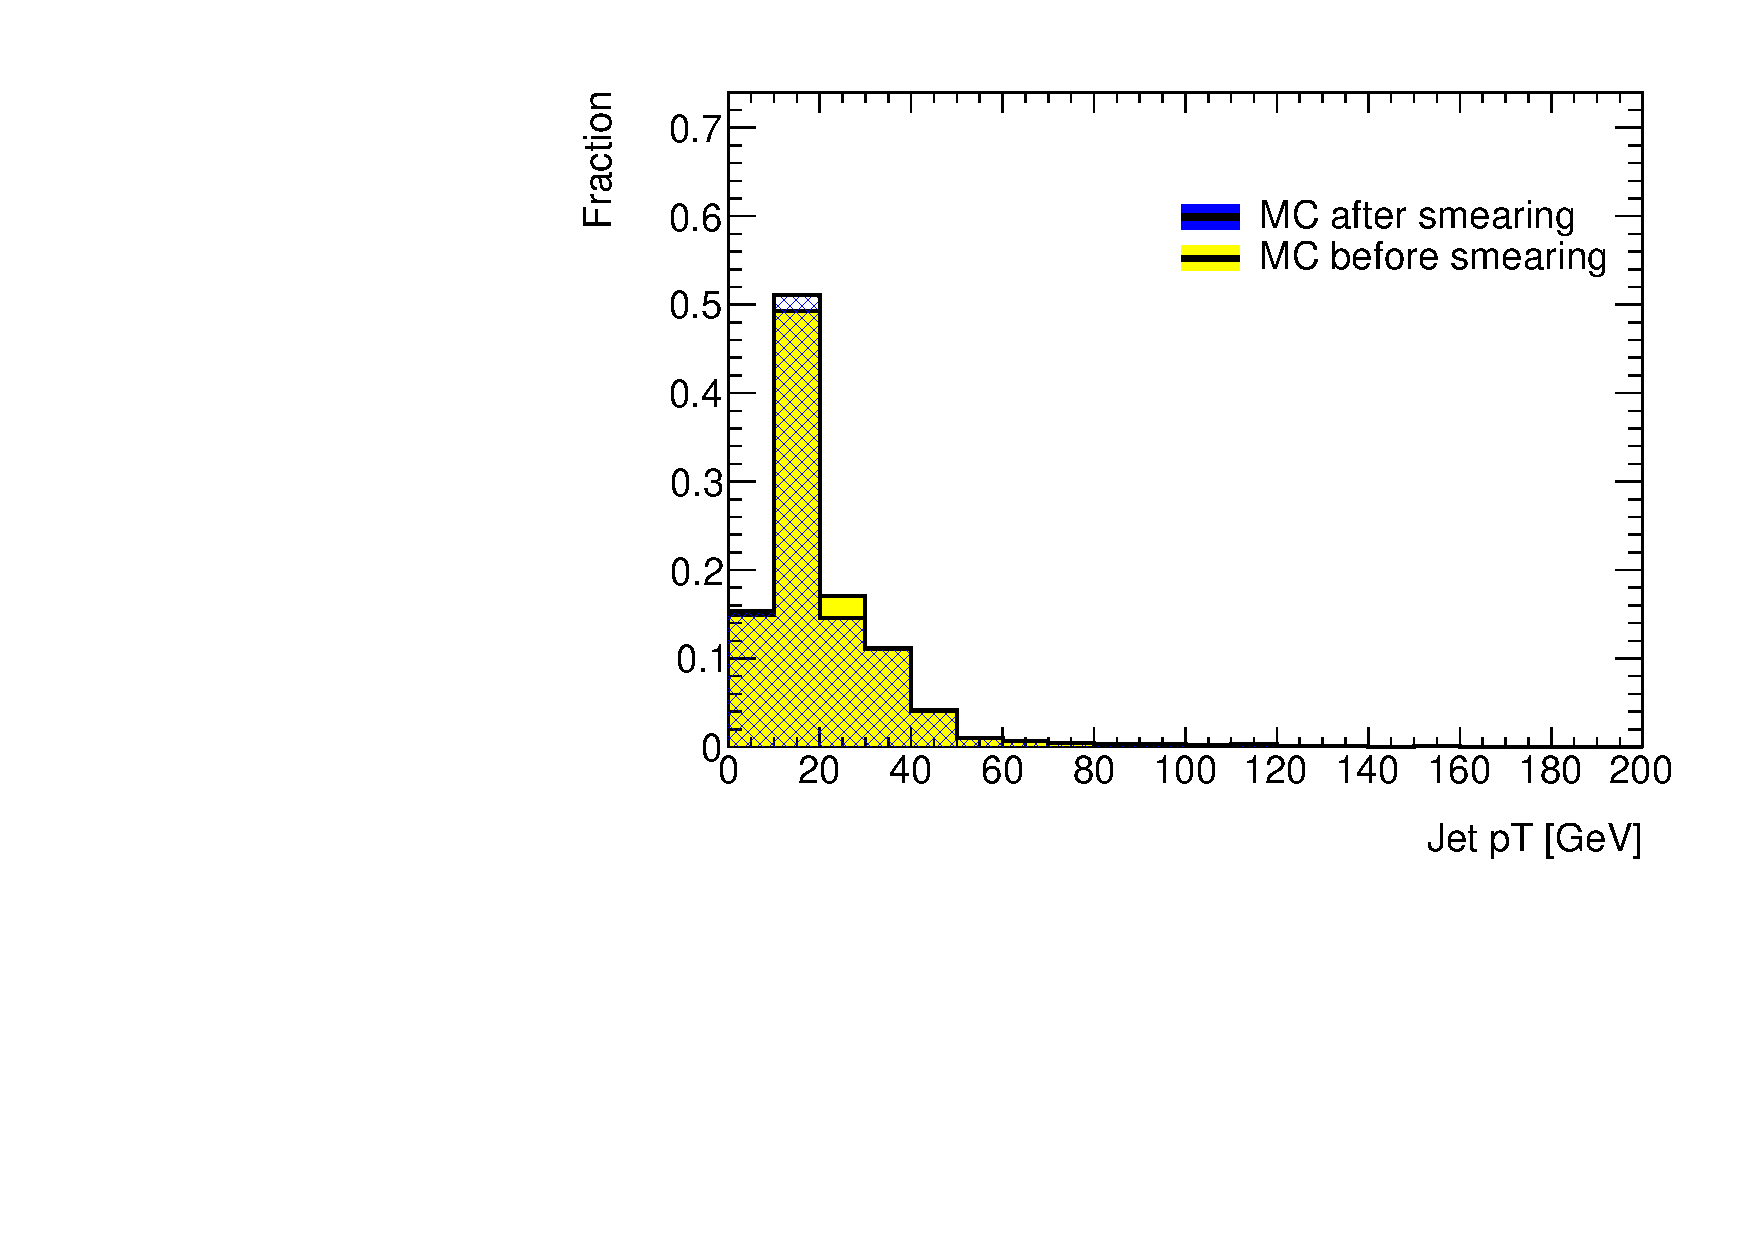
\includegraphics[width=0.53\figwidth]{testsmearingpt}
\caption[Influence of the Smearing on the transverse momentum]{The influence of the Smearing in momentum is shown}
\label{fig:testsmearingpt}
\end{subfigure}
\quad
\begin{subfigure}[b]{0.5\figwidth}
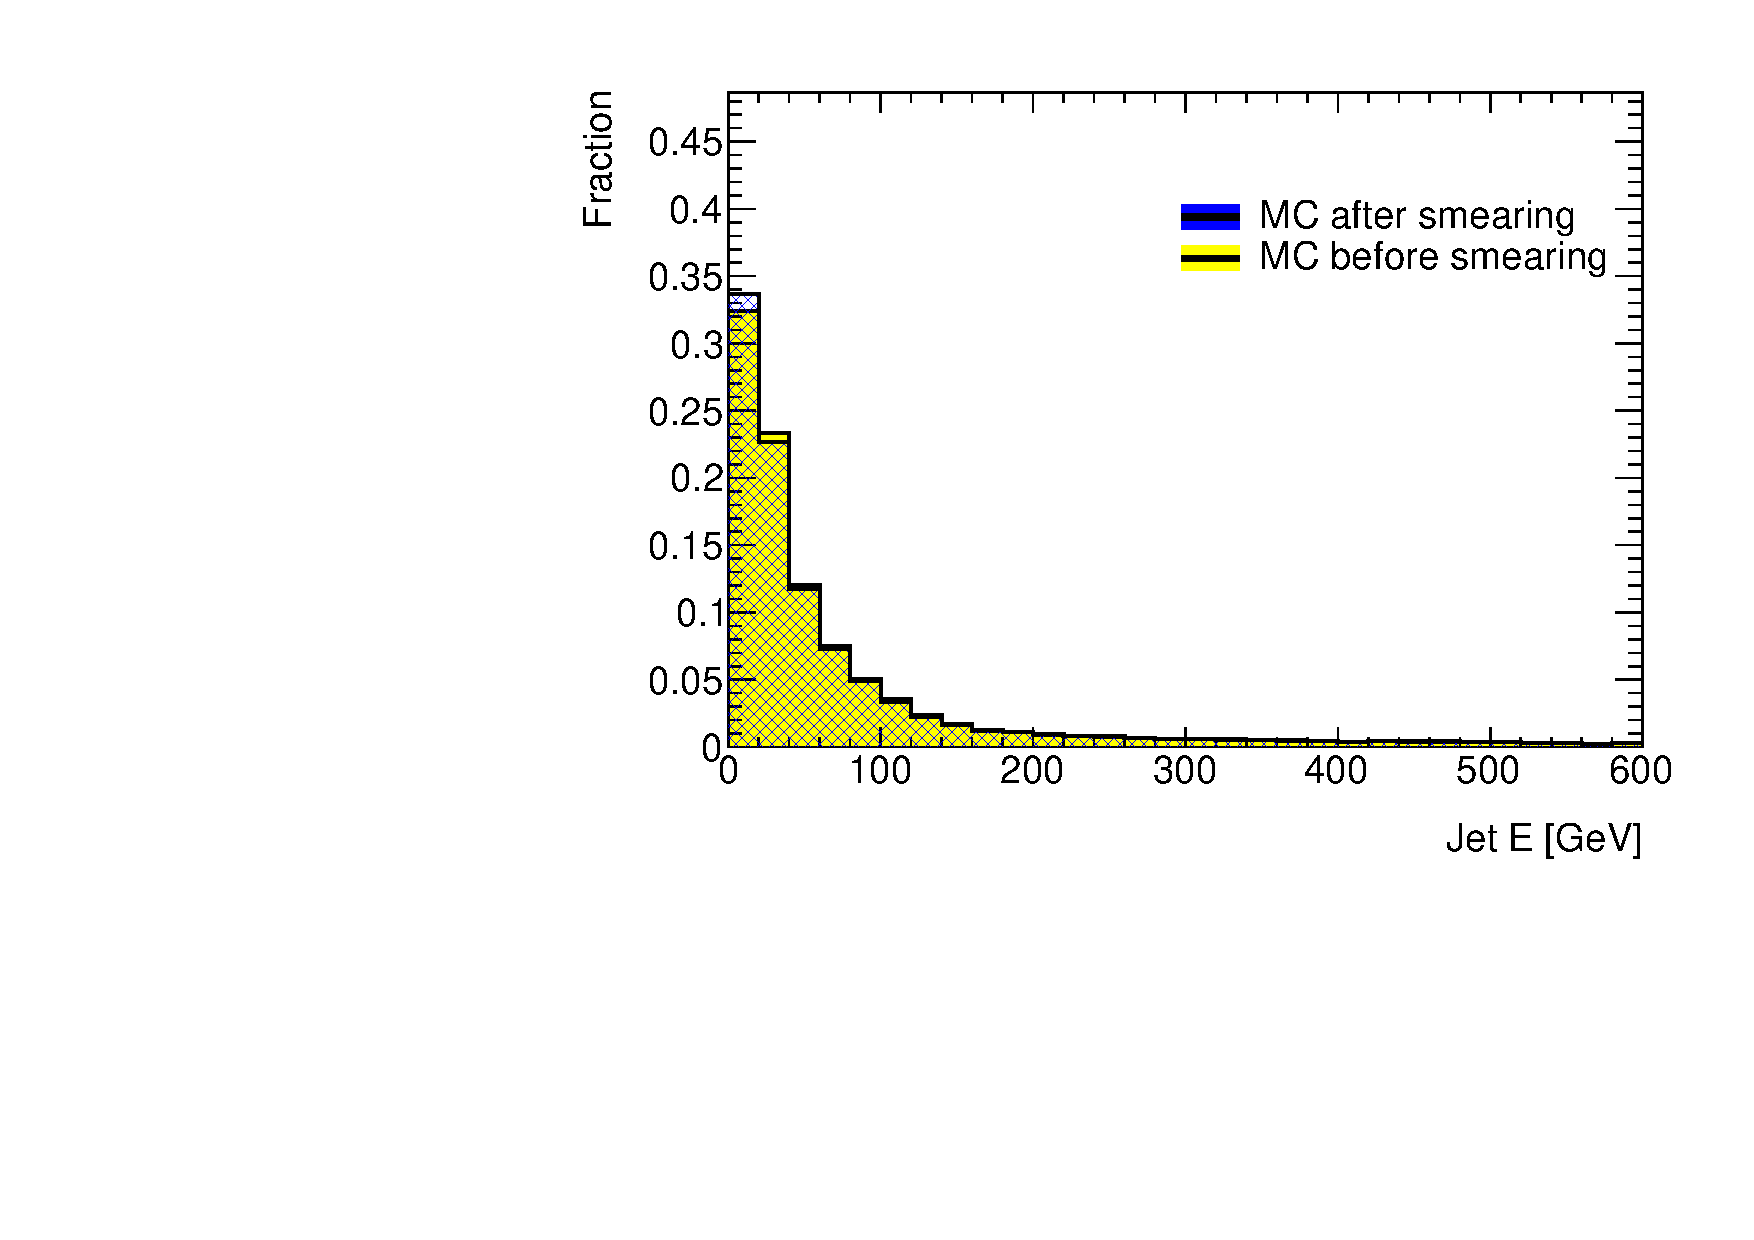
\includegraphics[width=0.53\figwidth]{testsmearinge}
\caption[Influence of the Smearing on the energy]{The influence of the Smearing in energy is shown}
\label{fig:testsmearinge}
\end{subfigure}
\caption[Jet Calibration and Smearing]{The figure demonstrates the results of calibration and smearing for Particle Flow jets. Figures (a) and (b) show the jet momentum and energy before and after scaling and figures (c) and (d) show the changes in the same variables for the smearing.}
\label{jetsmearingandcalibration}
\end{figure}


\subsection{The jet vertex tagger}

Due to the high luminosity at the LHC, pileup is a big challenge in ATLAS analysis. Therefore the rejection of pileup is an important part of analysis. One way to reject pileup is to calculate the jet-vertex fraction of each jet which is the fraction of momentum in the jet originating from the primary vertex. If one sets a minimum on this fraction pileup can be suppressed because jets that do not pass the criteria on their JVF are highly likely to be originating from pileup vertices. The Jet Vertex Tagger relates each jet to a vertex.


\subsection{Muon Calibration and Selection}

Muons are reconstructed using both the muon spectrometers and the inner detector. The information from both detector systems is combined to a single track.

Analogue to jets the muons also have to be calibrated properly. This section introduces all the important tools for muon calibration and gives a brief summary of the effects of the cuts and calibrations.
The first task of the muon tools is to determine whether a muon originated from the original vertex or has its origin in background noise (cosmic muons) or in some kind of secondary interaction.

The muons are requested to have $\pT > \SI{25}{\GeV}$ and a pseudorapidity of $|\eta| < \num{2.5}$. To reject the cosmic muon background further the muons are not allowed to have a longitudinal impact parameter to the primary vertex higher than \SI{3}{\mm}. 

The last requirement is added due to muons originating from heavy flavour quark decays.
To remove these muons an isolation criterion is implemented, namely the isolation tool. The tool is responsible for making sure that the sum of transverse momentum of the tracks around the muon candidate divided by the muons momentum is below \num{0.05}. [\ref{muoniso}]. The efficiency of this tool was checked with $Z \rightarrow \mu^+ \mu^-$ events providing a \num{97} \% in $\mu$ detection.

\begin{equation}
\frac{\sum_{\Delta R}\ensuremath{p_{\text{T},track}\xspace}{\ensuremath{p_{\text{T}, \mu}}\xspace}} < 0.05
\label{muoniso}
\end{equation}


The second part of the muon tools provides that the muon properties are correctly calibrated and smeared to make Monte Carlo and data match properly and to eliminate known weaknesses in the detector structure. Figure \ref{fig:testmuonpt} shows the muons transverse momentum before and after calibration in Monte Carlo. The changes are very minor.

\begin{figure}[h]
\centering
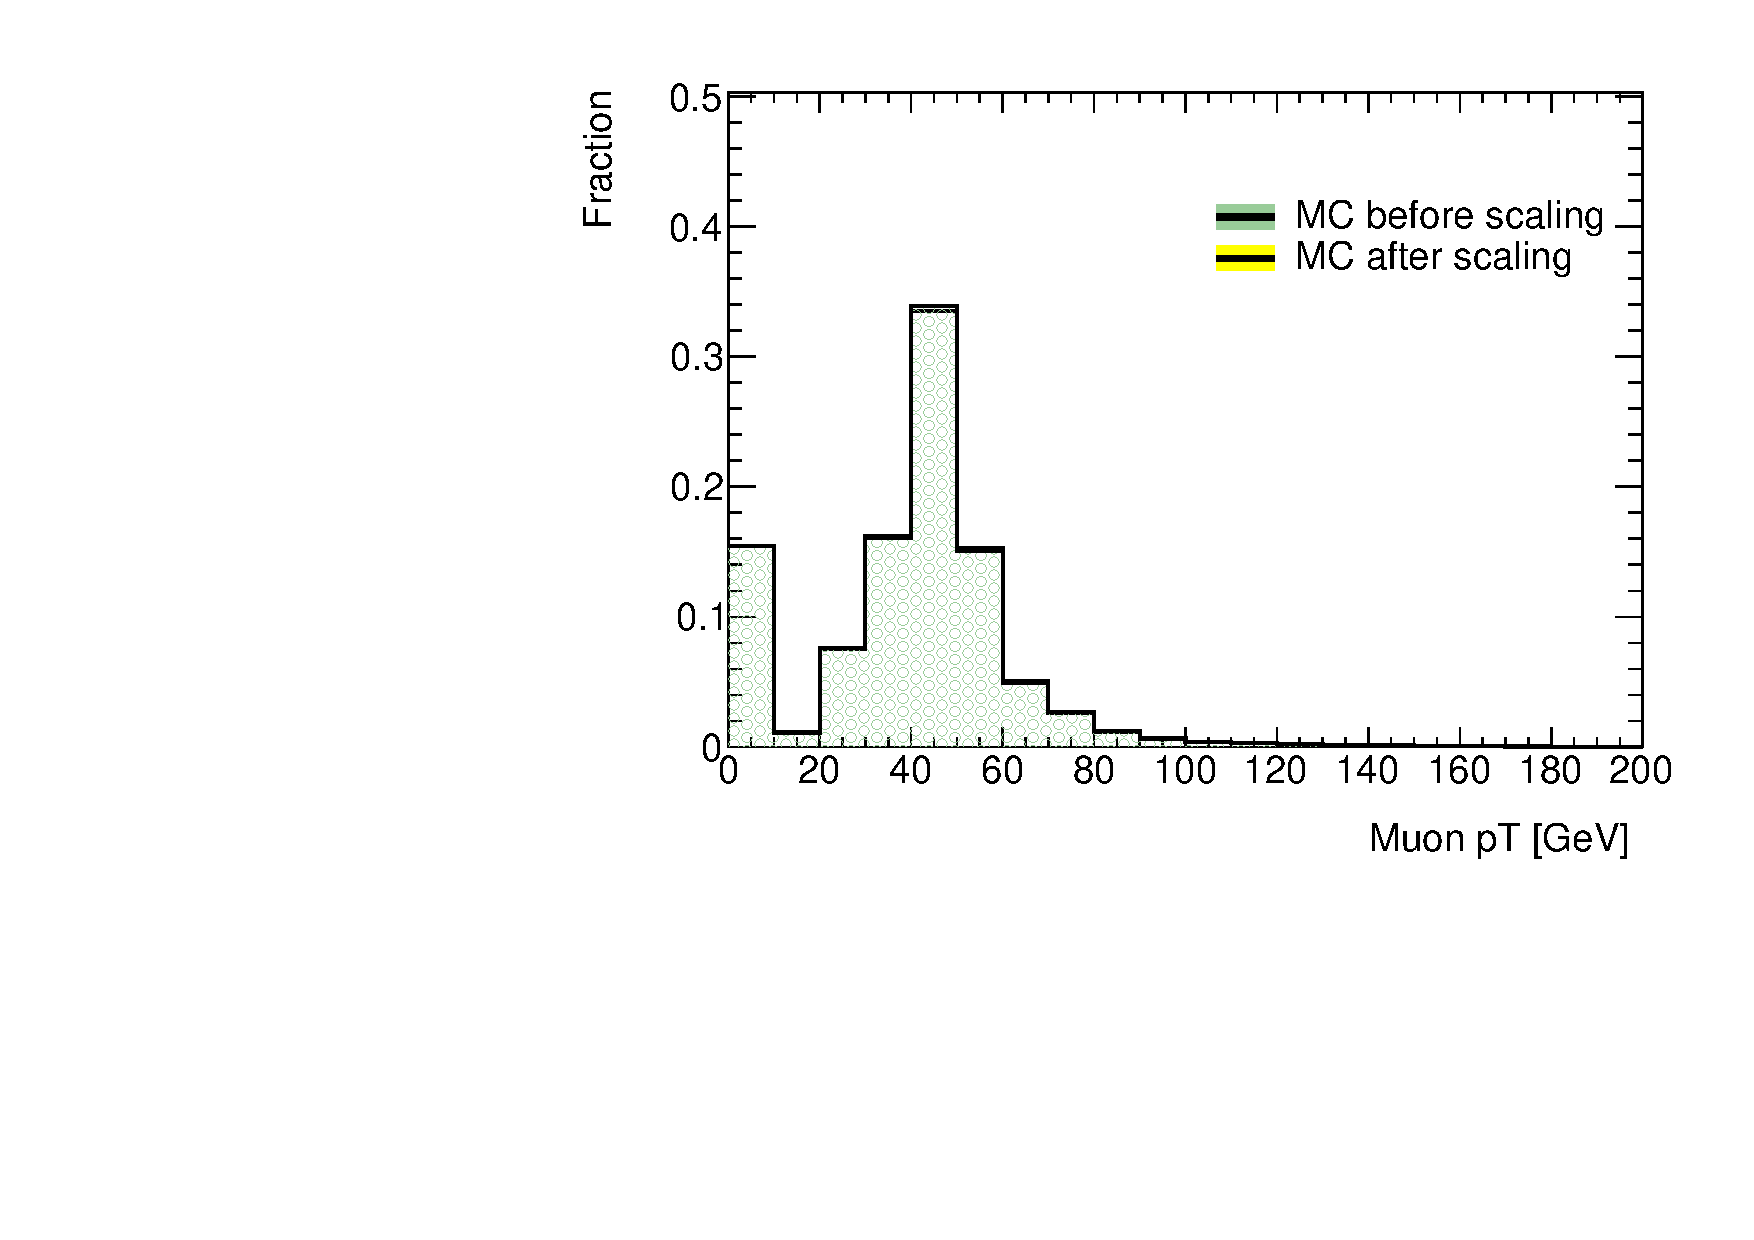
\includegraphics[scale=0.42]{testmuonpt}
\caption[Calibration and Smearing of the muon momentum]{Calibration and smearing of the muon momentum before any further cuts are applied. The changes are very minimal.}
\label{fig:testmuonpt}
\end{figure}

\subsection{Electron Calibration and Selection}


Electrons are detected by leaving a track in the inner detector and depositing close to all of their energy in the electromagnetic calorimeter. The reconstruction algorithm expects a calorimeter cluster with a deposited energy $E_T$ exceeding \SI{2.5}{\GeV}. This cluster has then to posses a matching track from the primary hard scatter vertex. The $\eta$ requirements are $|\eta|_{cluster} < 2.47$ with an exclusion of $\num{1.37} < |\eta| < \num{1.52}$ (calorimter barrel-endcap transition region).


The electron tools are very similar to the muon tools. There is a first group of tools and criteria to determine which electrons actually originate from the primary vertex and to distinguish those electrons from those originated in background and pileup events. The second group of tools calibrates electrons properties.

Electrons are as muons required to be isolated. The Isolation is based on a $\Delta R < \num{0.2}$ cone in the deposited energy and a $\Delta R < \num{0.3}$ cone around the track.

The electron calibration and smearing is exemplary displayed in figure \ref{fig:testelectronpt}. The impact of the scaling is significantly higher than for muons.

\begin{figure}
\centering
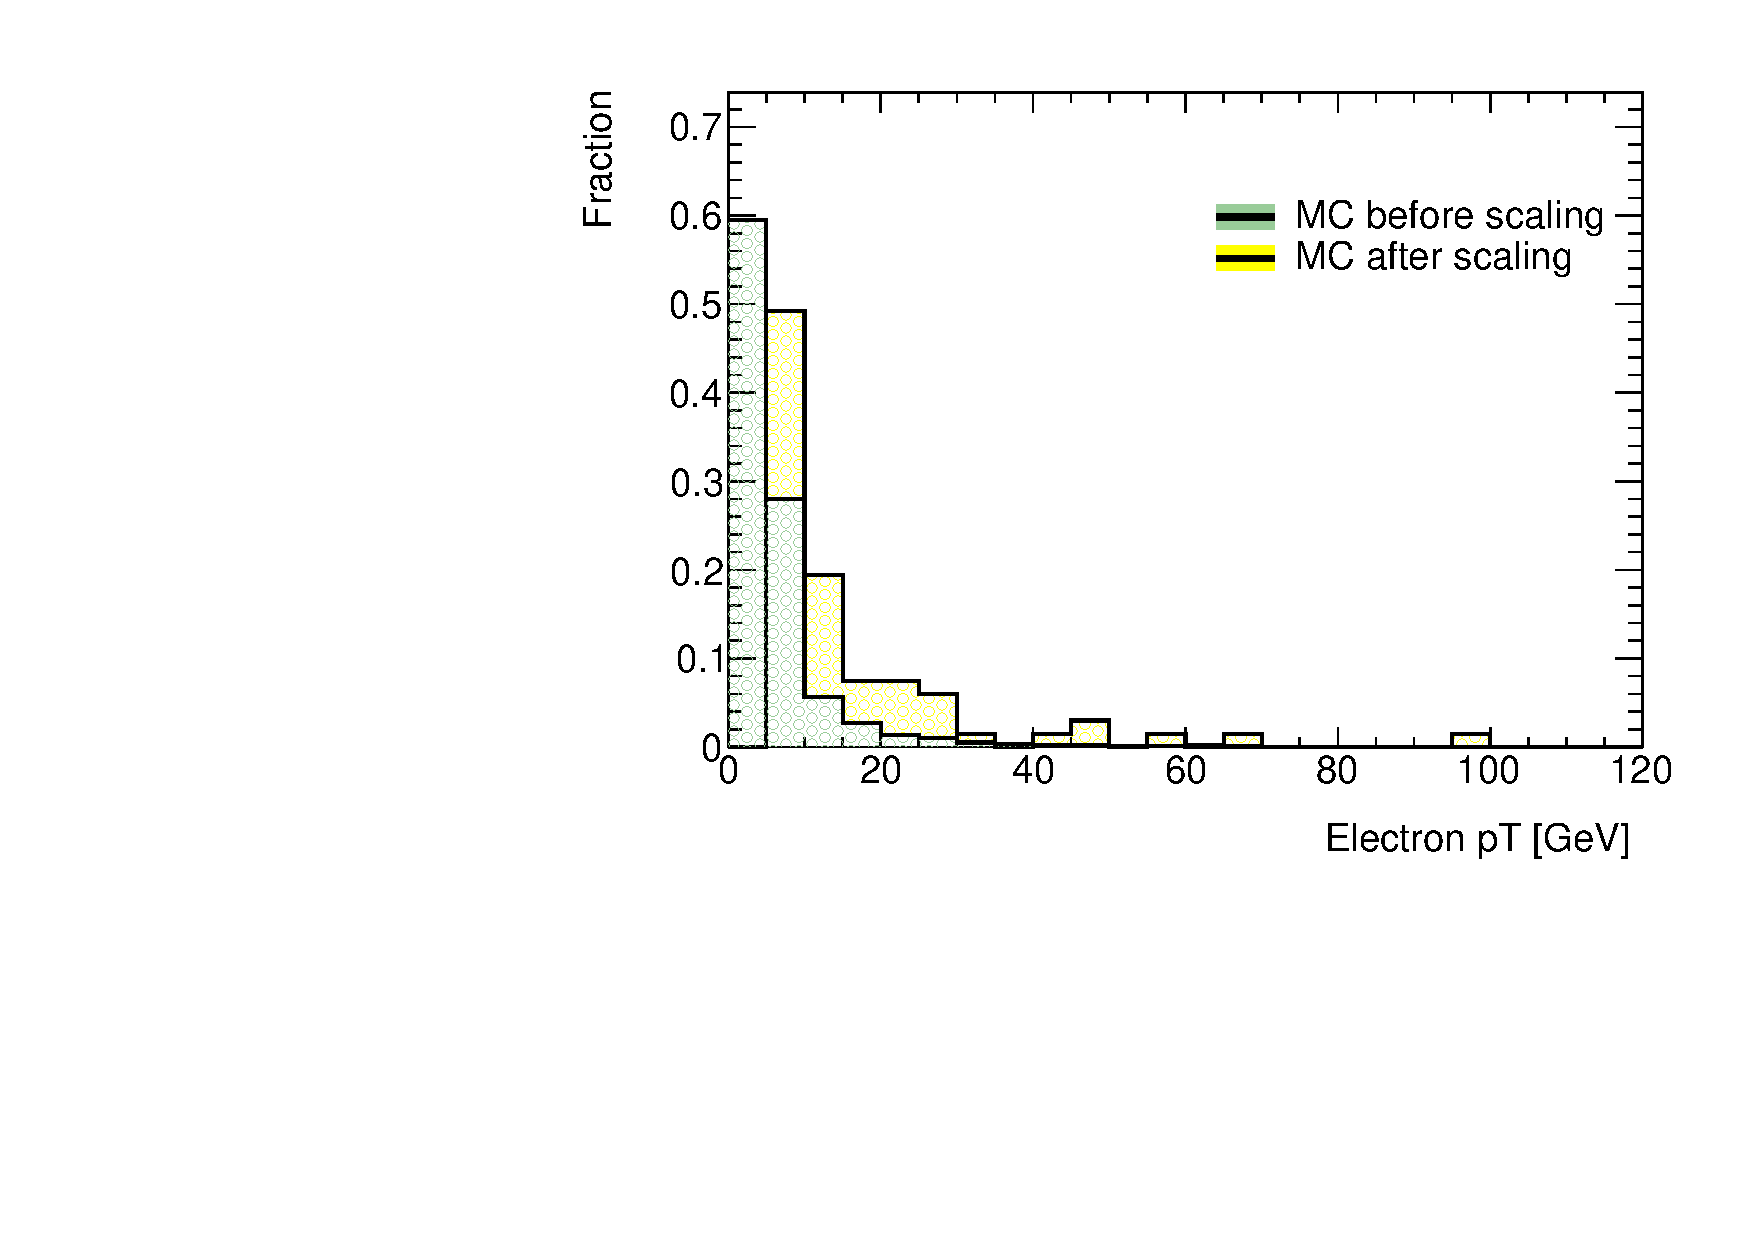
\includegraphics[scale=0.42]{testelectronpt}
\caption[Calibration and Smearing of the electron momentum]{Calibration and smearing of the electron momentum.}
\label{fig:testelectronpt}
\end{figure}